\documentclass[10pt,twocolumn,letterpaper]{article}

\usepackage{cvpr}
\usepackage{times}
\usepackage{epsfig}
\usepackage{graphicx}
\usepackage{amsmath}
\usepackage{amssymb}
\usepackage{comment}

% Include other packages here, before hyperref.

% If you comment hyperref and then uncomment it, you should delete
% egpaper.aux before re-running latex.  (Or just hit 'q' on the first latex
% run, let it finish, and you should be clear).
\usepackage[breaklinks=true,bookmarks=false]{hyperref}

% *** Custom commands

\newcommand\codeinline[1]{\texttt{#1}}  % alternatives: \mintinline{bash}{#1} or \mintinline{c++}{#1} or \textit{#1}

% *** Config

\cvprfinalcopy % *** Uncomment this line for the final submission

\def\cvprPaperID{****} % *** Enter the CVPR Paper ID here
\def\httilde{\mbox{\tt\raisebox{-.5ex}{\symbol{126}}}}

% Pages are numbered in submission mode, and unnumbered in camera-ready
%\ifcvprfinal\pagestyle{empty}\fi
\setcounter{page}{1}
\begin{document}

%%%%%%%%% TITLE
\title{Billys: The Bills Classifier}

\author{Bryan Lucchetta\\
{\small University of Padua}\\
{\tt\small bryan.lucchetta@studenti.unipd.it}
% For a paper whose authors are all at the same institution,
% omit the following lines up until the closing ``}''.
% Additional authors and addresses can be added with ``\and'',
% just like the second author.
% To save space, use either the email address or home page, not both
\and
Luca Parolari\\
{\small University of Padua}\\
{\tt\small luca.parolari@studenti.unipd.it}
}

\maketitle
%\thispagestyle{empty}

%%%%%%%%% ABSTRACT

\begin{abstract}
Everyone, sooner or later, has to face the messy world of bills. Every
month we get four/five or even more bills, coming from different
providers and about different expenses, with the duty to keep them
safe and easily available in case of need. This task can, even if can
be quite easy, is very boring for humans. Why don't let that a
computer do it! The main task of our application is, indeed, to put in
order this messy world.  In this paper we present our solution to this
problem. The solution is composed by simple steps, each of them solve
a different task like image dewarping, contrast/illumination
augmentation, textual feature extraction, classification. This simple
steps are then combined in a pipeline which manage the whole process.
\end{abstract}

%%%%%%%%% BODY TEXT

\section{Introduction}

The purpose of our work is to classify bills into some arbitrarily
defined categories\footnote{a.k.a., target names or classes}, that can
fit almost all bill categories. This targets should help the user to
better handle and organize bills for archiviation. We defined five
classes: \emph{Water}, \emph{Electricity}, \emph{Gas}, \emph{Trash and
  Recycling} and \emph{Telephone and Cable}. For treatability we
assigned to each class an integer from $0$ to $4$ is assigned,
respectively. Bills are the very foundamental component of the whole
application. A bill, or an invoice, is a commercial document issued by
a seller to a buyer, relating to a sale transaction and indicating the
products, quantities, and agreed prices for products or services the
seller had provided the buyer. In pratical terms, for us, a bill can
be a pdf file or an image (even a a camera taken image) to process.

The task itself is very complex and can lead to a messy and
unmantainable solution. For this reason we develop a robust and well
structured pipeline with the aim to face some of the main problems,
described below.
\begin{itemize}
  \item Image dewarping. Camera taken image are usually not directly
    processable by an optical recognition tool. In order to perfomr
    the OCR we have to preprocess the image and rotate, resize and
    strech the image.
  \item Contrast/illumination augmentation. Also the
    illumination/contrast of an image can be a nasty problem for an
    OCR tool, as it needs a clear distinction from written text and
    other stuff in order to perform well.
  \item Optical Character Recognition. The OCR can be a very delicate
    point, as the application performances depends on how the OCR
    extracts data from images.
  \item Text preprocessing. An huge amout of details can be extracted
    from the OCR, but surely not all of them are relevant for
    application's purposes. We need to disregard them for good
    results.
  \item Feature classification. At the end, our need is to classify
    the given object. This is a complex task as document data can be
    very different and very similar at the same time.
\end{itemize}

In the following sections we present our work and we face the problems
described above. We start from related works in Section
\ref{sec:related-work}, where we discuss about our starting
point. Then, in Section \ref{sec:dataset}, we present our dataset and
some information about the context of the data we used. After that, in
Section \ref{sec:proposed-method}, we show adopted solutions and
describe smart ideas we used in order to solve the core problem. We
then explore the pipeline and all its components in order to present
full details of what we have done. In Section \ref{sec:experiments},
we also show experiments and fails we have done before getting nice
results. We conclude then with future works and possible enhancements
that for concreteness we excluded from this presentation and we wrap
up with some considerations about the work in Section
\ref{sec:future-works} and \ref{sec:conclusion}, respectively.

\section{Related Work}
\label{sec:related-work}

During our researches, we did not found works that perform this
particular task. However, we found interesting works about different
aspect that we had to face when developing this work.  First of all we
take into account the image dewarping problem, that previously has
faced by \cite{Improvingcamera-based} with his project
\cite{mobile-ocr}. Their proejct is based on the experiments conducted
by \cite{recoveringhomography}.  Secondly, we had to perform text
extact from images. In order to do that we relied on Tesseract
\cite{Tesseract} wich is a popular open-source OCR tool developed by
Goggle. The last major step that we had to take into account was the
classification phase, which could be performed by a Naive Bayes
Classifier, TODO set references.

\section{Dataset}
\label{sec:dataset}

When dealing with machine learning applications, data are a
foundamental aspect to keep in mind: no data, no party. In fact, in
order to get quite accurate results, a lot of data are needed. For our
application, public domain datasets are very rare, mostly because the
sensible data contained inside each document. For this reason, before
starting with the ``low level'' application we had to collect the
data.

We collected two different dataset that we used to satify our needs
and testing our application during its stages. This two dataset are
described below.

\paragraph{Main Dataset}
\label{par:main-dataset}

The \emph{main dataset} is the first dataset we collected. It is
composed by nearly one thousand bills, where the majority of them are
camera taken photos, while a small part of them are pdfs (either
scanned or the original file).

We tried to keep images with no perspecitive distorsion or other
effects and to exclude the background as much as possibile, because
these corrections are made in a prevoius pipeline steps. See the full
pipeline in Figure \ref{fig:pipeline}.  In this way we could use the
assumption that documents are already dewarped and we could train the
classifier without being influnced by the preprocessing steps. Even if
we tried to keep the illuminance as good as possible, we included in
the preprocessing phase the brightness enhancing.

While the dataset could be a nice starting point, it has one big
problem: documents do not variate so much. In fact,
\begin{itemize}
  \item documents come from a small number of people, so headers are
    really similar from one document to another;
  \item providers are almost the same, because bill were collected
    from the same local zone;
  \item classes are umbalanced, because some type of bills are less
    frequent than others.
\end{itemize}

The Table \ref{table:main-dataset} shows the composition of our
dataset.

\bgroup
\def\arraystretch{1.5}%
\begin{table}[!h]
  \begin{center}
    \begin{tabular}{p{1.5cm} p{1.2cm} p{1.2cm} p{3cm}}
      \hline
      Categories  & Number of Documents & Number of Providers & Providers \\ \hline
      \emph{Telephone and Cable} & 403 & 9 & Vodafone, Wind, Tre, Wind Tre, Telecom, TIM, Tele 2, Fastweb, Teletu \\
      \emph{Electricity} & 276 & 6 & Green Network, Servizio Elettrico Nazionale, Etra, Enel, Edison, Hera \\
      \emph{Gas} & 202 & 4 & Sorgenia, Ascotrade, Etra Energia, Hera \\
      \emph{Water} & 123 & 3 & Etra, Alto Trevigiano Servizi, Hera \\
      \emph{Garbage} & 45 & 1 & Savno \\ \hline
      \textbf{Total} & 1048 & 19 &  \\ \hline
    \end{tabular}
  \end{center}
  \label{table:main-dataset}
  \caption{Main dataset composition.}
\end{table}
\egroup

\paragraph{Warped Dataset}
\label{par:warped-dataset}

The \emph{warped dataset} is instead the second dataset we collected
consists of nearly one hundred and fifty camera taken photos of our
home bills, as in the main dataset, but in this case they are taken
with perspective distorsion, rotation and with parts of the
background. With this dataset we are able to test the full
pipeline. The results obtained with this dataset and with the full
pipeline are reported in Section \ref{sec:experiments}.

\section{Proposed Method}
\label{sec:proposed-method}

The task itself is very complex and can lead to a messy and
unmantainable solution. For this reason we develop a robust and well
structured pipeline with the aim to face some of the main problems,
described below.

\begin{itemize}
  \item Image dewarping. Camera taken image are usually not directly
    processable by an optical recognition tool. In order to perfomr
    the OCR we have to preprocess the image and rotate, resize and
    strech the image.
  \item Contrast/illumination correction. Also the illumination of an
    image can be a nasty problem for an OCR tool, as it needs a clear
    distinction written text and other stuff in order to read that.
  \item Optical Character Recognition. This can be a very delicate
    point, as the application performances depends on how the OCR
    extracted data from images.
  \item Text preprocessing. An hige amout of details can be extracted
    from the OCR, but surely not all of them are relevant for
    application's purposes. We have to disregard them.
  \item Feature classification. At the end, owr need is to classify
    the given object. This is a complex task as document data can be
    very different and very similar at the same time.
\end{itemize}

To resolve all this problem we prososed the pipeline reported in
figure \ref{fig:pipeline}. We choose to add an Optical Carachter
Recognition in our project because we thought that using a simple CNN
to classify the bills could bring some problems like, what are the
behaviuor of an CNN in front of a new unseen bill about another
supplier. Another reason is the fact that a CNN need a lot of examples
(huge dataset) to be trained and because we have only "few" exaples we
prefered to try another approach. So we chose Tesseract to extrapolate
all the text inside a bill and then classify the bill accordingly to
all the text extracted. In this way we think that a text classificator
is much more stable in predicting the bill's type of a new unseen
example, because in an unseen new bill the words extrapoleted are in
general the same as the words extracted from the bills included in the
main dataset. Once we have chosen to include an OCR all the rest of
the pipeline is built upon the major drawback already known for OCRs,
like image preprocesing (Page dewarping and Brightness \& Contrast
Enhancer). Obtained all the text from the bills we need to preproccess
also the extrapoleted text before the final step. This part is
important for excluding the frequent words like articles and verbs
often used wich are not important for the final classification. In
what following we will dive into the details of the designed pipeline.

\begin{figure*}[h]
  \centering
  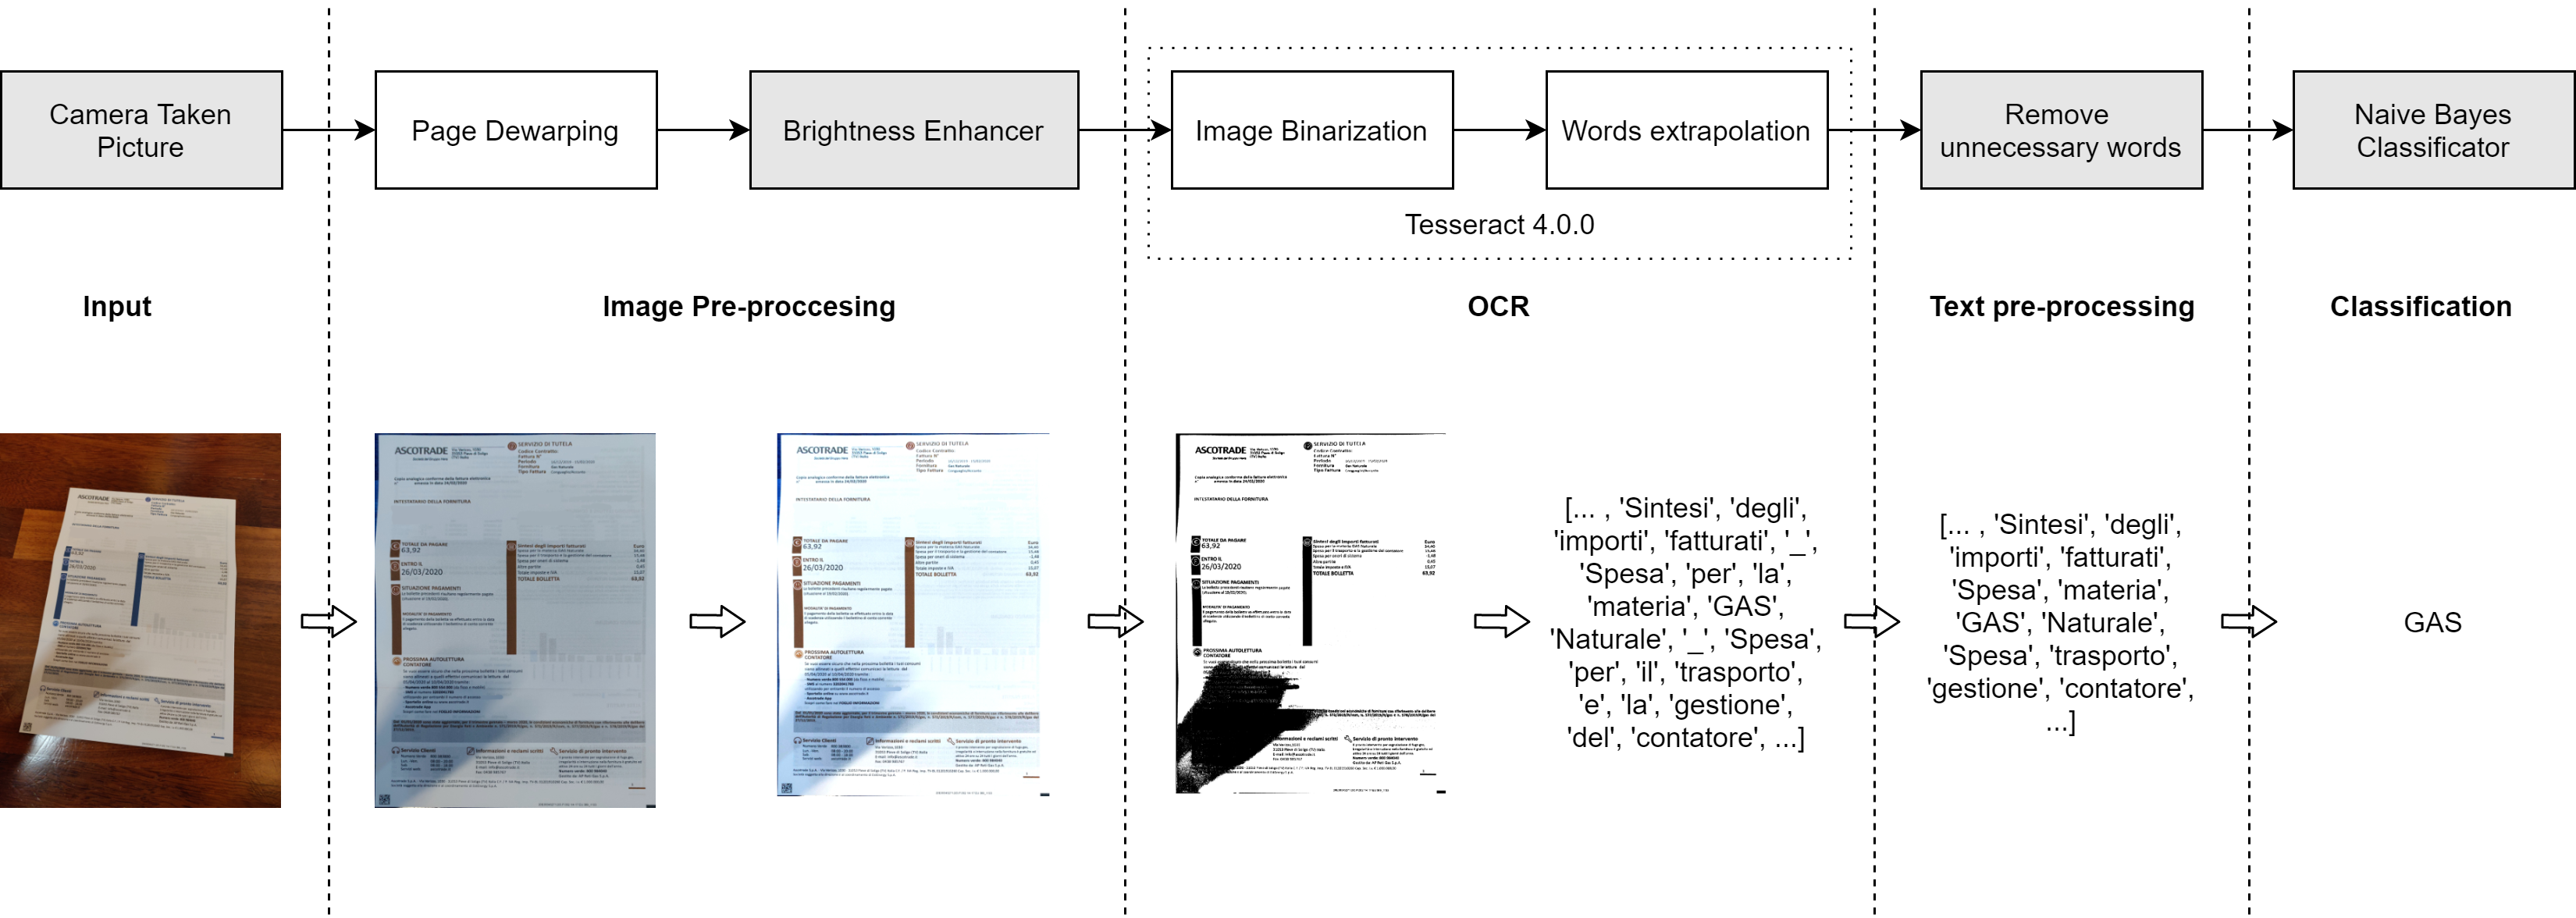
\includegraphics[width=1.0\textwidth]{images/pipeline.png}
  \caption{Our pipeline}
  \label{fig:pipeline}
\end{figure*}

\subsection{Image pre-processing phase}

The image preprocessing phase is in charge of adjusting all the aspect
of a mobile camera taken photos. This includes brightness and contrast
adjustments, dewarping, skew correction and others. The first task of
our pipeline infact is try to recover a flatbed scanned document from
a camera taken photos. For this task we used the work done in
\cite{mobile-ocr} wich uses an Xcenption Neural Network
\cite{xception_NN} to perform this task, with appreciable results
according to the article. In figure \ref{xception-architecture} is
reported the Xception architecture used in this application coming
from the work done in \cite{Improvingcamera-based}. We have observed
that in some experiment, that involve the second dataset which
consists of mobile camera taken photos of bills in extreme conditions,
the network doesn't correctly adjust the homography of some document
contained in the dataset. The last step of the image pre-processing is
the correction of the brightness and constrast of the image. This is
done because there are critical photos that could arise many problem
for the OCR phase and this problems are be better exaplined in the
Experiment section.

\subsubsection{The Xception Neural Network}

The dewarping phase is completly based on the work done in
\cite{mobile-ocr}. Accordingly to the autor, the recovery of the
homography of a mobile camera taken photos of a document is delegated
to a Xception Neural Network. According to the paper \cite{xception}
this architecture relies heavily on prior efforts in the Inception
architecture wich first demonstrated the advantages of factoring the
convolutions into multiple branches operating successively on channels
and then on space. It is entirely based upon the Residual Connections
and Depthwise separable convolutions. For the Depthwise separable
convolutions advantages we refer to the article
\cite{https://towardsdatascience.com/a-basic-introduction-to-separable-convolutions-b99ec3102728}
and for Residual Connections we refer to
\cite{https://towardsdatascience.com/residual-blocks-building-blocks-of-resnet-fd90ca15d6ec}.

\begin{comment}
--- Depthwise separable convolutions SUMMARY ---

unlike spatial separable convolutions (wich is used to reduce the computational complexity of a single convolution operation involving one kernel by dividing it into two smaller kernels), depthwise separable convolutions work with kernels that cannot be “factored” into two smaller kernels. The depthwise separable convolution is so named because it deals not just with the spatial dimensions, but with the depth dimension (the number of channels) as well. Similar to the spatial separable convolution, a depthwise separable convolution splits a kernel into 2 separate kernels that do two convolutions: the depthwise convolution and the pointwise convolution. We refer to this article  that exaplain better this two operations in the details with an example.

--- Residual Connection SUMMARY --- 
accuracy increases with increasing number of layers. But there is a limit to the number of layers added that result in accuracy improvement. So, if neural networks were universal function approximators then it should have been able to learn any simplex or complex function. But it turns out that, thanks to some problems like vanishing gradients and curse of dimensionality, if we have sufficiently deep networks, it may not be able to learn simple functions like an identity function. Now this is clearly undesirable.

You can skip the training of few layers using skip-connections or residual connections. This is what we see in the image above. In fact, if you look closely, we can directly learn an identity function by relying on skip connections only. This is the exact reason why skip connections are also called as identity shortcut connections too. One solution for all the problems!
\end{comment}

The used Xception neural network is trained over 1.5M synthetic images
dataset. It uses Adam optimization method in combination with the
L1-loss to predict the 4 corner points of the distorted document
image. Then given this 4 obtained points from the Xception neural
network, the homography matrix H is computed using Direct Linear
Transforma (DLT) algorithm. The network is made of 36 convolution
layers and a total of 20,823,344 trainable parameter.

\begin{figure}[h]
	\centering
	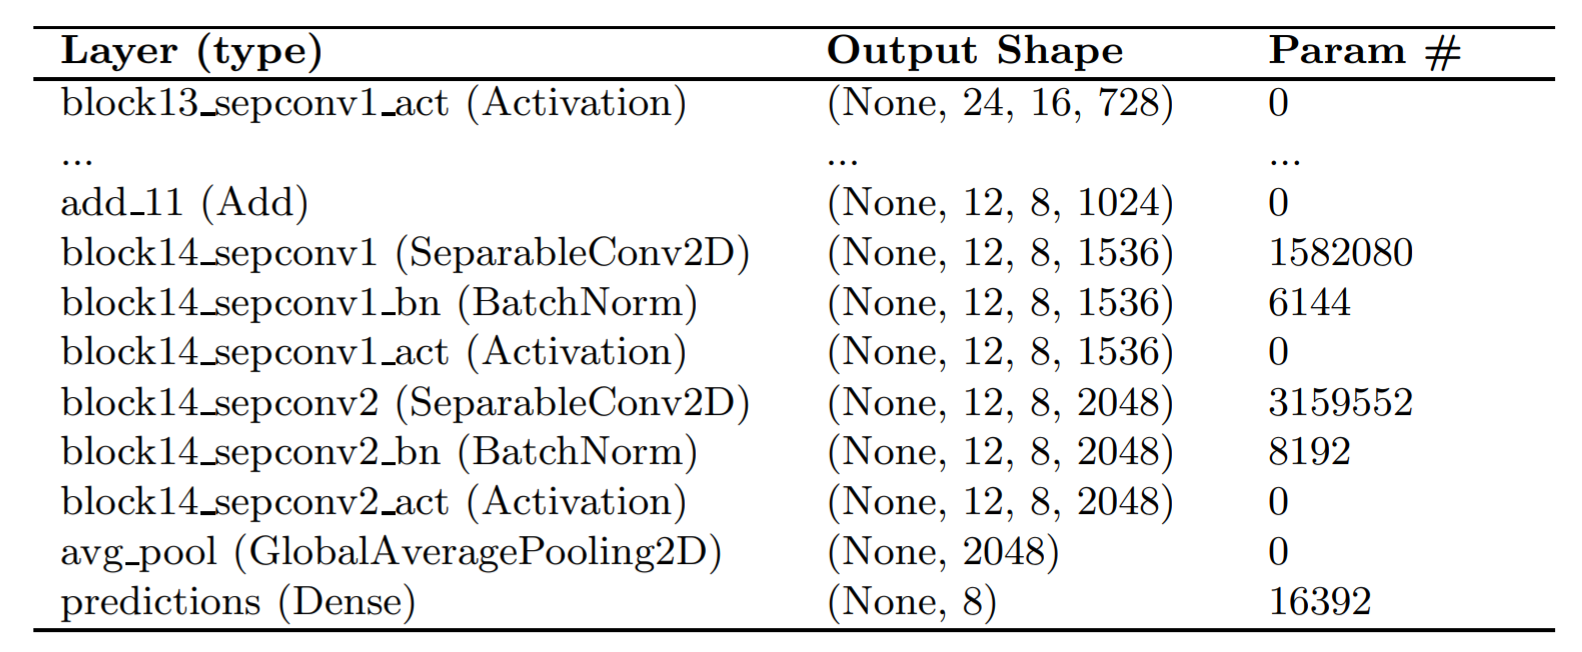
\includegraphics[width=0.48\textwidth]{images/xception-architecture.png}
	\caption{The Xception architecture used in this work}
	\label{xception-architecture}
\end{figure}

\subsection{Optical Character Recognition}

As we have seen this phase is delegated to Tesseract, which is a
open-source OCR to extract all the words containded in a
image. Tesseract is developed from Google and it is publically
available on GitHub.

\subsection{Text Preprocessing}

The text preprocessing phase is an important task that may occur
immediatly after the textual features extraction from images. The aim
of this task is mainly to preprocess the plain text coming from images
in order to remove non-relevan features: pratically, it transform the
text into a more digestible form so that machine learning algorithms
can perform better.

The implementation of this step follows some very simple ideas for
text preprocessing. Indeed, we just normalize the text into its base
form. The inner pipeline for this phase is composed by atomic steps,
described below. Note that for this task, the execution order of some
steps really matters, so we ordered them for better performances.

\begin{enumerate}
  \item \textbf{To lowercase}: the first step for the text normalization is to
    remove differences from uppercase and lowercase letters.
  \item \textbf{Remove accented characters}: accented chars, specially in
    italian, are often used. However for our task they are not relevant
    and the OCR may also miss them, so we decided to exclude them from
    the principle and to represent words with their non accented
    versions.
  \item \textbf{Remove punctuaction}: also the punctuaction do not really
    matters, and indeed cannot say anything on the class of the bill
    that we are considering, so we decied to remove them.
  \item \textbf{Remove numbers}: bills can be full of numbers and we can find
    them under many forms, as, for example, dates, identifiers,
    furniture comsumption, and so on. However, also numbers cannot say
    anything about the bill class, so they were removed and replaced
    with the keyword \codeinline{<num>}, which instead can be more
    informative as in a bag of words represents the number of numbers
    in a bill. For this case, we decied to do not completely remove
    the information but to keep only its condensed version.
  \item \textbf{Remove stopwords}: in order to obtain the most informative
    textual representation of a bill we had to remove also
    insignificat words like stopwords. Stopwords are words that can be
    used frequently in phrases, so in the context of representing the
    bill class, an article isn't informative. Stopwords are remove
    with the help of the \emph{Natural Language Toolkit}, available as
    a python package: \emph{nltk}. NLTK provieds a collection of
    stopwords, that can be easily downloaded with
    \codeinline{nltk.download('stopwords')}, and then, with
    \codeinline{nltk.corpus.stopwords.words('italian')} we can obrtain the
    localized version of the stopwords and perform the removal.
  \item \textbf{Remove shortwords}: By means of experiments we discovered that
    the OCR phase, under certain (bad) conditions, returns parts of
    words, usually very smaller. We empirically found that by removing
    this ``shortwords'', we could improve performances.
  \item \textbf{Lemmatize}: lemmatisation (or lemmatization) in linguistics is
    the process of grouping together the inflected forms of a word so
    they can be analysed as a single item, identified by the word's
    lemma, or dictionary form.\footnote{\href{
        https://en.wikipedia.org/wiki/Lemmatisation}{
        https://en.wikipedia.org/wiki/Lemmatisation}}. With
    this step, indeed, we tried to group words together in order to
    simplify the classification phase. However, we noticed that this
    step do not improve the performance and it can also produce worst
    results as it tries to group wrong words retrieved from the OCR.
  \item \textbf{Tokeinze}: at the end of the preprocessing we create a list of
    words (Tokenization), that can be easily represented by in a
    vectorized form.
\end{enumerate}

\subsection{Features Classification}
\label{subsec:classification}

The features classification is itself a core step, needed for the real
bills classification. Indeed, the pipeline steps before the features
classification can be viewed as a giant image preprocessing step, with
the goal to preprare a nice subset of features to be used in the
classifier.

Regardless of the chosen implementation for a classifier, textual
features need a transformation in order to be handled: we need to
transform text into numerical feature vectors. In order to do this, we
can use the \emph{bag of words} technique, that is based on the
following strategy:

\begin{itemize}
  \item Assign a fixed integer id to each word occurring in any
    document of the training set (for instance by building a
    dictionary from words to integer indices).
  \item For each document $i$, count the number of occurrences of each
    word $w$ and store it in $X[i, j]$ as the value of feature $j$,
    where $j$ is the index of word $w$ in the dictionary.
\end{itemize}

Once we have the bag of words we can analyze words occurency in order
to extract frequencies. We cannot rely on occurrencies because longer
documents will have higher average count values than shorter
documents, even though they might talk about the same topics. To avoid
these potential discrepancies it suffices to divide the number of
occurrences of each word in a document by the total number of words in
the document: these new features are called \emph{Term
  Frequencies}. Another refinement on top of \emph{tf} is to downscale
weights for words that occur in many documents in the corpus and are
therefore less informative than those that occur only in a smaller
portion of the corpus. This downscaling is called \emph{Term Frequency
  times Inverse Document Frequency} (\emph{tf-idf} for brevity).

Now, we are ready to train the classifier in order to predict a bill
category. For completing this task we proposed using a
``deterministic'' classifier, that relies on words frequency and a
ground truth vocabulary. The deterministic classifier is based on the
simple idea that each document category has a small subset of words
that are very relevant for the classification. Indeed, we have
arbitrary defined the vocabulary that specifies what words we expect
to find in a document based on its category. Then, the classifier
applies a simple algorithm, which works as follows:

\begin{itemize}
  \item Compute the frequency of each word in a given bill;
  \item For each word, if it is a relevant word\footnote{A word $w$ is
    a relevant word if it is contained in some keyword $kw$ and the
    longest common subsequence between $w$ and $kw$ is at least $|kw|
    - 1$.}, sum its contribution to the aggregate sum of the category
    of that word;
  \item Return the class which has more contributes.
\end{itemize}

The Figure \ref{table:determnistic-classifier-dict} shows an example
of the vocabulary (italian version) we used to perform bills
classification, how we can see, it is very small and effective.  On
the contrary, one could think to automatically generate the
vocabulary: this could be a valid option! See the Section
\ref{sec:future-works}.

Obviously the deterministic classifier is not the only way to perform
the classification task, in fact, we experimented also a Naive Bayes
Classifier. See Section \ref{subsec:naive-bayes-classifier}.

\bgroup
\def\arraystretch{1.3}%
\begin{table}[!h]
  \begin{center}
    \begin{tabular}{p{2cm} p{5cm}}
      \hline
      Class & Keywords \\ \hline
      Water & acqua, idrico, depurazione, fognatura, trevigiano \\
      Garbage and Recycling & spazzatura, immondizia, riciclato, riciclo, rifiuti, rifiuto, savno, igiene, ambientale\\
      Gas & gas, naturale \\
      Electricity & luce, energia, tensione, potenza, chilowatt, elettricita, elettrico, elettrica, green, enel, edison \\
      Telephone and Cable & telefonia, telefonate, telefonico, chiamate, canoni, fibra, internet, ricaricabile, ricarica, cellulare, navigazione, telecom, vodafone, tim, fastweb, wind \\ \hline
    \end{tabular}
  \end{center}
  \label{table:determnistic-classifier-dict}
  \caption{Example of one vocabulary for the deterministic classifier.}
\end{table}
\egroup

\section{Experiments}
\label{sec:experiments}

\subsection{Dewarping or not?}

As already widely discussed in the articles
\cite{Improvingcamera-based} and \cite{recoveringhomography} the
dewarping phase (also the deskew phase) is essential to improve the
performance of Tesseract. We could confirm this fact with this
experiment: we proccessed the same image, one time without dewarping
it and the next time with the dewarping correction. If we highlight
the extracted words in the two corresponding images we could see that
there is a huge difference. Infact if we take a look at the figure
\ref{dewarping-experiment} we could see that in the image without the
dewarping correction the highlighted word are less than the same image
dewarped and also the output is more precise and with fewer
unneccesary random words that Tesseract could try to "guess". We could
report that the extracted text for the non-dewarped image contains 708
words but a lot of them are blank spaces, while for the dewarped image
the amout of extacted words are 491 but the output in this case is
more precise and there are fewer blank spaces.

\begin{figure}[b]
  \centering
  \includegraphics[width=0.48\textwidth]{images/dewarping-experiment.png}
  \caption{Difference with and without dewarped text extraction}
  \label{dewarping-experiment}
\end{figure}

Moreover we tried to do the classification of the photos contained in
the second dataset, which is made of bills photos with perspective
distorsion and a lot of background, with Naive Bayes Classificator
trained on the main dataset and without dewarping the photos. In this
case we obtained an accuracy of 0.64 instead of 0.95 obtained with the
same dataset but with the dewarping phase also enabled in this last
case. This experiment confirm that the dewarping phase is an important
task when dealing with OCR application and in that specific task it
has improve the perfomance in terms of accuracy of nearly 30\%.

\subsection{Camera taken illuminance quality}

We have noticed during our expiremets that we have poor performances
in the OCR phase if the mobile taken photos isn't correctly
illuminated. Tesseract OCR, wich is the application designated for
extracting the text of our bill in our application, already apply
internally an image pre-processing step, trying to binarize the image
for the later text extraction phase. The problem of this
pre-processing step of Tesseract arise when the taken photos have a
bad illumination or there are shadows present on it. Infact we could
see in the example reported in figure
\ref{bright-constrast-experiment} that if we take a poor illuminated
photo of a bill and we print the pre-proccesing output of Tesseract we
can noticed that there are completly white areas on the pre-processed
photos and the binarization is inverted. For this reason if we try to
increase the brightness of the image we could see that the peformance
are better. Infact if we take the same image as the example but this
time we increase the brightness we could notice that the
pre-proccessed image of Tesseract is better, without too much area
invisibles and also without the inversion of the binarization of the
image. With this improvemets also the text extaction phase is more
precise and accurate and it could extract all the words where before
was contained in the white areas. For this reason we have inserted in
the pipeline a "Brightness Enhancer" for all the mobile taken photos
(the jpg format), because we have seen that also if the image is
already correctly illuminated and costrasted, even if we apply the
enhancer, the performance are the same. We could confirm also this
hyphothesis by stating that the accuracy performance obtained in class
(wich was the more problematic in terms of image illumincance) with
and wothout the brightness enhancer increase from 0.94 to 0.99. We set
manually the amount of brightness to be added, but it could be learned
automatically with a deep learning model. Another improvement could be
also increasing the contrast with an apropriate values depending on
the image.

\begin{figure}[h]
  \centering
  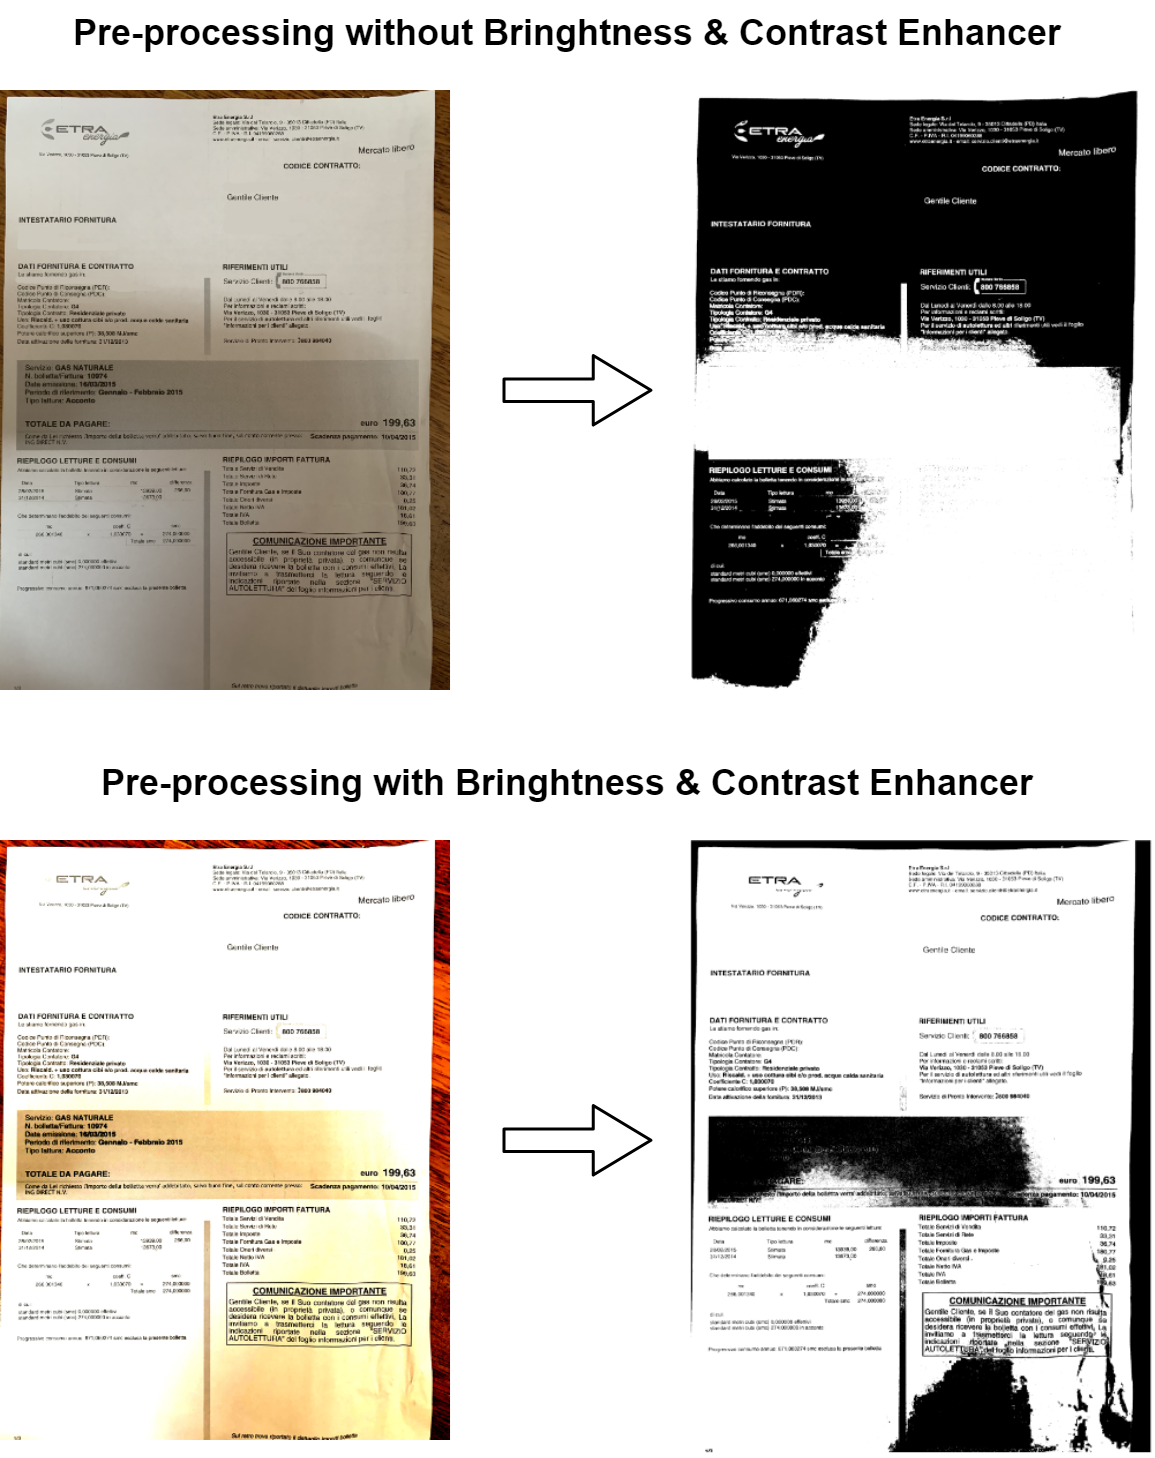
\includegraphics[width=0.4\textwidth]{images/bright-contrast-experiment.png}
  \caption{Difference with and without brightness and contrast enhancer}
  \label{bright-constrast-experiment}
\end{figure}

\subsection{Naive Bayes Classifier}
\label{subsec:naive-bayes-classifier}

The deterministic classification strategy proposed in Section
\ref{subsec:classification} is not the only feasible way. There are
many machine learning algorithms applicable with text classification:
one over the other is Naive Bayes.

The Naive Bayes classifier, unlike the deterministic classifier, comes
from the family of simple probabilistic classifiers based on applying
Bayes' theorem with strong (naive) independence assumptions between
the features. Indeed, it calculates the probability of a certain word
to be seen in a document and it uses that probability in
classification phase for predicting the document class. For our task
we need the Multinomial Naive Bayes classifier, as we have to predict
multiple classes, not only two.

Due to the definition of our problem, this type of classifier
is probabily an overkill: it bases the predicted target on all the
text provided to the classifier. Under our domain, documents are very
likely to be similar for most of their parts and we have only few
interesting words for each document that differs. Also, bills contains
huge amount of non-relevant data for our application like marketing
banners, disclaimers, formal opening of letters, and so on. Another
problem we had, as described in Section \ref{sec:dataset}, is the
problem of the headers: we can have two bills about different
categories with same header (same user data), or bills about same
category with different headers (different user data).

We tried to test this two different ideas with another dataset
composed by unseen bills with different headers and providers, and we
discovered that the two perform quite the same. However, we must
underline that this third dataset was composed by very very few data,
so the results are not reliable.

\paragraph{Results}

The Table \ref{table:classifiers-comparison} shows a comparison
between the performance of the main and the warped dataset (described
in Section \ref{sec:dataset}), for the Naive Bayes classifier trained
on our main dataset and the deterministic classifier. In the second
dateset, we enabled and disabled the dewarphing phase to see the
difference in performance with this task.

\begin{table}[!h]
  \begin{center}
    \begin{tabular}{lll}
      \hline
      Classifier & Accuracy & Support \\ \hline
      \textbf{Main Dataset} \\
      \small Without dewarping phase\\
      \; \; Naive Bayes & $0.99$ & $1047$ \\
      \; \; Deterministic & $0.99$ & $1047$ \\ \hline
      
      \textbf{Second Dataset} & & \\
      \small Without dewarping phase \\
      \; \; Naive Bayes & $0.59$ & $129$ \\
      \; \; Deterministic & $0.40$ & $129$ \\ 
      
      \small With dewarping phase \\
      \; \; Naive Bayes & $0.98$ & $129$ \\
      \; \; Deterministic & $0.88$ & $129$ \\ \hline
    \end{tabular}
  \end{center}
  \label{table:classifiers-comparison}
  \caption{Accuracy comparison between Naive Bayes classifier and
    deterministic calssifier.}
\end{table}

\section{Future Works}
\label{sec:future-works}

The task offers a infinite list of related works that can be done in
order to improve results and extends our ideas. We list below some of
possible future works.

\begin{itemize}
  \item Enhanced Text Preprocessing. Our text preprocessing is not
    sophisticaded, instead it is composed by the necessary steps in
    order to get a decent classifier. An enhance on text preprocessing
    could be the header removal. Under the bills domain, headers are
    composed of extremenly non-relevant data, that could be discarded
    with a vocabulary of names or something similar.
  \item Automatic Vocabulary Building. For concreteness, we manually
    built the vocabulary used in the deterministic classifier, instead
    one could let the machine generate it. In fact, our approach has
    some drawbacks: the application tends to be static, but mainly,
    the vocabulary can miss some relevant words. A well configured
    vocabulary automatic building can surely perform better wrt the
    manual one.
\end{itemize}

\section{Conclusion}
\label{sec:conclusion}

From this experience we can first of all conclude that data are the
real core of nowdays applications, specially for the machine learning
ones: having a good dataset is, we would say, the hardest part of the
whole project, bacause all results depends on the data you have. We
also learned a lot about image preprocessing and feature extraction
from images: the only fact that a simple rotation or perspective
distortion can catastrophically change what features can the OCR
extract, was very desturbing. We spent a lot of time on image
preprocessing as in a concrete context users do not pay much attention
on the way they make photos. Another part were we dedicated lot of
time was the classification part. In fact, that part was one of the
harder because the complexity of the pipeline: a small change on the
contrast preprocessing phase leads to a significant change on the
classification stage. 

However, we are really happy with this experience and we know that the
work is only at the beginning.

{\small
\bibliographystyle{ieee_fullname}
\bibliography{egbib}
}

\end{document}
